\subsection{Performance Comparison}
\label{subsec:performanceComparisonDiscussion}

%\textbf{COHEN: How did the program performance compare to its selected standard?} 
%\textbf{Did the program demonstrate good performance?}
%\textbf{Is the programs performance different from predictions?} 
%\textbf{Did you learn what you wanted from the experiments?}

The best route set, having four routes, constructed by the proposed method (SSO), is illustrated in Fig. \vref{fig:bestRouteSet4}. Comparison of ACO and SSO concerning the average produced results is presented in Table \vref{table:performanceComparison_ACOSSOBEST}. The best, worst, and median results with the standard deviation can be found in Appendix \ref{appendixC}, Table \vref{table:performanceComparison_ACOFull}. SSO is identical to the plain ACO implementation, but with the additional attributes inspired by PSO and BCO, in addition to the memory attribute. By using an otherwise identical algorithm enables directly comparing the performance of the two algorithms. 

As one can see in Table \vref{table:performanceComparison_ACOSSOBEST}, SSO performs better than ACO concerning the performance criteria. Observing Figure \ref{fig:acovssso}, ACO performs worse than SSO already in the first iteration. One reason for this difference is because the ants in ACO are without the memory attribute. This feature enables the ants to ``remember'' which nodes it has visited within the same route set. Adding this attribute makes the ants favor nodes not visited over nodes already visited, to increase the probability that all nodes within the route set are visited at least once. Constraint \vref{itm:criteriaConnectedGraph} specifies that the route network must be connected, and without the memory function, ACO will produce less solutions satisfying this constraint. This again makes ACO produce more route sets that will be discarded, and thus not evaluated. %The lack of this attribute will thus prevent more (possible better) route sets being explored.  

 \begin{figure}[H]
    \begin{center}
    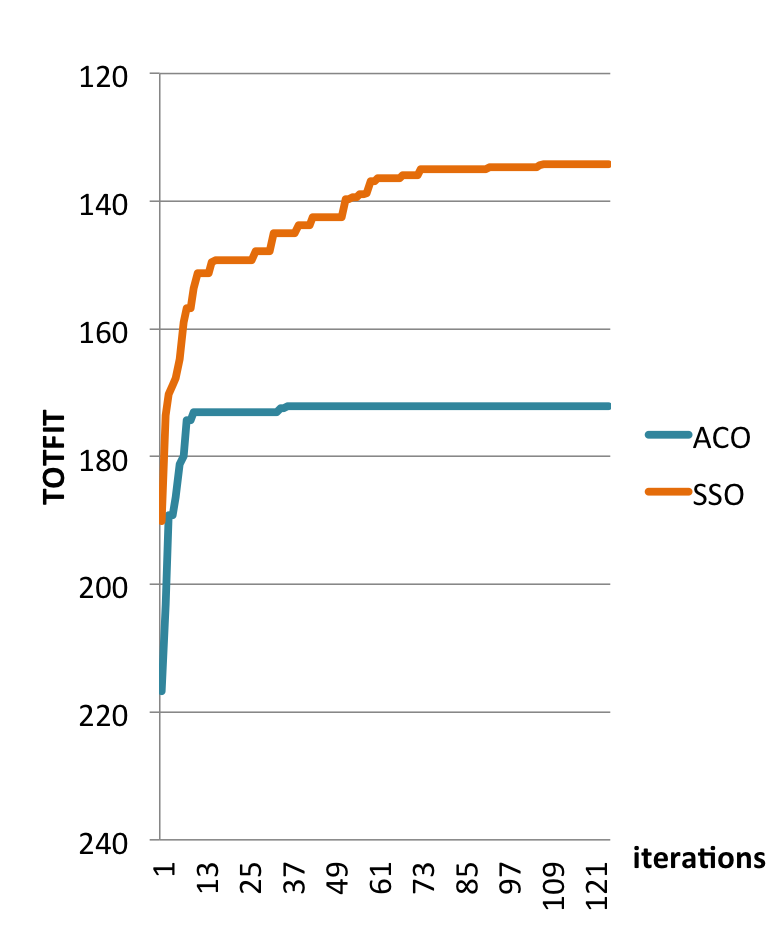
\includegraphics[width=2.5in]{assets/acovsssoNEW.png}
    \end{center}
    \caption{Evolution of TOTFIT for ACO and SSO }
    \label{fig:acovssso} 
\end{figure}

%Kan hente noe info fra setningen over?
Another reason for the difference in performance is due to the fact that ACO has, as mentioned, a known shortcoming of entrapment in local optima. This disadvantage is demonstrated in Figure \ref{fig:acovssso}, which shows the average growth in the $TOTFIT$ value for each iteration. (In this figure, both algorithms are run 10 times. For each iteration the average $TOTFIT$ value for each run is recorded.) As one can observe, the ACO implementation manage to find good solutions fast. Before any distinct pheromone trail is laid, the ant's choices are more random and thus they perform a broad search in the environment. This randomness will decrease over time as the pheromone trails become more distinct. Because pheromone evaporate over time, shorter paths will be favored over longer paths simply because shortest paths takes shorter time. Observing Fig. \ref{fig:acovssso}, after approximately 35 iterations the amount of pheromone on the initial first best routes continue to increase, and the short paths become excessively attractive to the following ones. This again unable the next ants to explore possible better solutions. ACO's approach is good enough when the problem to be solved is to be optimal. However, for the UTRP the problem to be solved is the attempt of finding the best possible solution. The evaluation of the route set as a whole is done after each iteration, and this evaluation will determine how good the produced route set is. Because of the lack in rewarding the best route sets in the classic ACO, there are possibility in ``informing'' the ants if they are converging towards a local optimum.

As one can see, the proposed SSO method manage to get out of this inconvenience, continuing to explore better solutions in the late iterations. Observed in the parameter settings experiment, extracted in Table \vref{table:pm2_inEvaluation}, the additional $CA$ and $AF$ parameters inspired by PSO and BCO respectively both improved the $TOTFIT$ value. 

\begin{table}
    \centering
    %\hspace*{-0.5cm}
    \begin{tabular}{|l|l|l|l||c|}
    \hline
    Parameter & $CA$ & $AF$ & $p_b$ & $AVG(TOTFIT)$ \\
    \hline
    $CA$ & \textbf{0\%} & 10\% & 0.0 & 105.66\\
    ~ & \textbf{25\%} & 10\% & 0.0 & \textbf{103.597}\\
    \hline
    $AF$ (and $p_b$) & 10\% & \textbf{0\%} & \textbf{0.0} & 105.747 \\
    ~ & 10\% & \textbf{5\%} & \textbf{1.3} & \textbf{102.579}\\
    \hline
    \end{tabular}
    \caption {Caption}
    \tiny
    \begin{itemize}[noitemsep]
    \item[ ] $AVG(TOTFIT)$ : Average produced Total Fitness function
    %\item[$^1$:] On average \% of the iterations of each run did not create any ants that satisfied the initial Constraint \ref{itm:criteriaConnectedGraph} described in Section \vref{sec:algoConstraints}.
    \end{itemize}
    \label{table:pm2_inEvaluation}
\end{table}
\emph{\color{blue}Mulig denne må kuttes ned, vi sier jo dette i parameter settings experimentet.}

The $AF$ attribute is added to the proposed method to reward edges in the best route sets with more pheromone. This feature was partly influenced by \citet{tripathi09} and \citet{sedighpour14}, which demonstrated that rewarding the best solution found so far improved their proposed algorithm. Rewarding the best solution may also be seen as the recruitment function in BCO. If an artificial bee in BCO has produced a good route set it can ``recruit'' other nest-mates, and thus inform the others that a good route set is found. This process inspired to add the ``following'' feature to the proposed method. After the route sets are evaluated, an amount of the best ants with the best route sets is selected to be followed in the next iteration. The same amount of ants will follow the same routes and thus create the exact same route set. This gives the edges in the best route sets more pheromone, and thus distinct edges with much pheromone (because they are walked by many ants, given the short path) from edges that are better concerning the performance criteria. Our method performed best with a relatively small amount of followers, but giving these edges a larger amount of pheromone.  Rewarding edges in a large amount best route sets will result in over appreciating too many edges, which again will unable to distinct edges in good route sets from edges in the best route sets. 


\emph{\color{blue}Samme med denne}

However, when the pheromone values on the best edges so far become too great it will unable SSO in exploring new (possible) better solutions. The attribute $CA$ was added to the proposed method to resolve from this path. $CA$ denotes the amount of ``crazy ants'' which will explore edges randomly, regardless of the pheromone value on the edge. $CA$ is inspired by how the particles in PSO explore solutions. In PSO, a parameter called Inertia Weight gradually decrease to prevent the particles from drastically changing directions, and thus becoming more organized in the late iterations. \citet{kechagiopoulos14} proved that the PSO shows great performance. To balance the global search by the ``crazy ants'' in the late iterations the Inertia Weight inspired by PSO is added to the proposed method. The Inertia Weight in the proposed method denotes the amount of crazy ants in the beginning of each run, and the amount of ``crazy ants'' decrease in line with the parameter. Decreasing the inertia weight in PSO may suffer from low global search ability at the end of the run, and thus the possibly of getting stuck at a local optima. However, in the proposed method the ``crazy ants'' are not searching towards the best known solution, and will thus prevent the same disadvantage. This may be due to the fact that the attribute enables an amount of ants to explore undetected better solutions when pheromone trails becomes too great.
\newline 

%The PSO algorithm enables exploring in early iterations and becoming more organized in the late iteration.
%The parameter is added to balance the local and global search, preventing the particles from drastically changing directions. However, the best global known solution the particles are drawn against may, similar to ACO, be a (possible) local optimum. This parameter can thus enable the algorithm to break out of a (possible) local optima. 

In order to determine the performance of the proposed method, it is compared to approaches published in the literature. Table \vref{table:performanceComparison_4}, the results of the SSO, having four routes, are compared with route sets published in the literature. As one can observe in Table \vref{table:performanceComparison_4},  $d_{unsat}$ is 0, similar to all other approaches. The theoretical best value of for this criteria is 0, which reflects no passenger have to transfer more than 2 times. All approaches, except \citep{mandl79, kidwai98, chakroborty02}, performs better concerning the $d_0$, $d_1$ and $d_2$ criteria. However, the route set constructed by SSO has a better $ATT$ compared to all route sets constructed by the other approaches. This is due to how the $TOTFIT$ value is calculated. The calculation of $TOTFIT$ is, as mentioned, the sum of $F1$, $F2$ and $F3$. As described in \vref{sec:f1}, a weight parameter, $\sigma$, is used to control the importance of $F1$, $F2$, and $F3$. In the proposed method, $\sigma$ is sat to favor $F1$, which is directly linked to a low $ATT$. Demonstrated in Fig. \vref{fig:mandlWithTT}, when traveling from Node 7 to Node 14, SSO will choose to transfer from Route 4 to Route 3, which has a travel time of 20 minutes including a transfer penalty of 5 minutes. The $F2$ parameter is concerned whether the proposed method has a high $d_0$, denoting a minimum number of transfers. If $F2$ was favored over $F1$, the route set would get a lower score and thus not be considered as the best route set. This is because Route 1, which have a direct route from Node 7 to Node 14 have a travel time of 27 minutes. It is worth mentioning that the the proposed method will not select $F1$ unconditionally. As seen in the produced results, a high amount of $d_0$ is still an important factor when determining the best route set, but the selection of the best route set will be determined concerning the ratio between the two parameters. As mentioned in the motivation, citizens often prefer private transportation because of the decreased travel time when no detours is needed. Then again, another important issue concerning passenger satisfiability, is the issue of not needing to change vehicles during a trip. Whether a passenger would travel travel direct with a larger travel time versus transferring and thus decrease the travel time, is a matter of preferences. As you can see in all the approaches published in the literature including the proposed method, you will have to choose one at the expense of the other. One can argue back and forth on the importance of each criteria. We believe that in the modern urban city, a minimum travel time is an important factor. People should have a small travel time as an option if time is limited. As mentioned, the produced route network also possess a relatively high amount of direct routes, giving passengers opportunities to choose direct routes if it is desired. %And reflecting the average travel time of the best route set produced by the proposed algorithm, the direct travels are not very long. %jeg er litt usikker på om jeg er på villspor her
%In the end, it is up to each individual passenger choosing what is most convenient for them. 

\begin{figure}[H]
    \begin{center}
    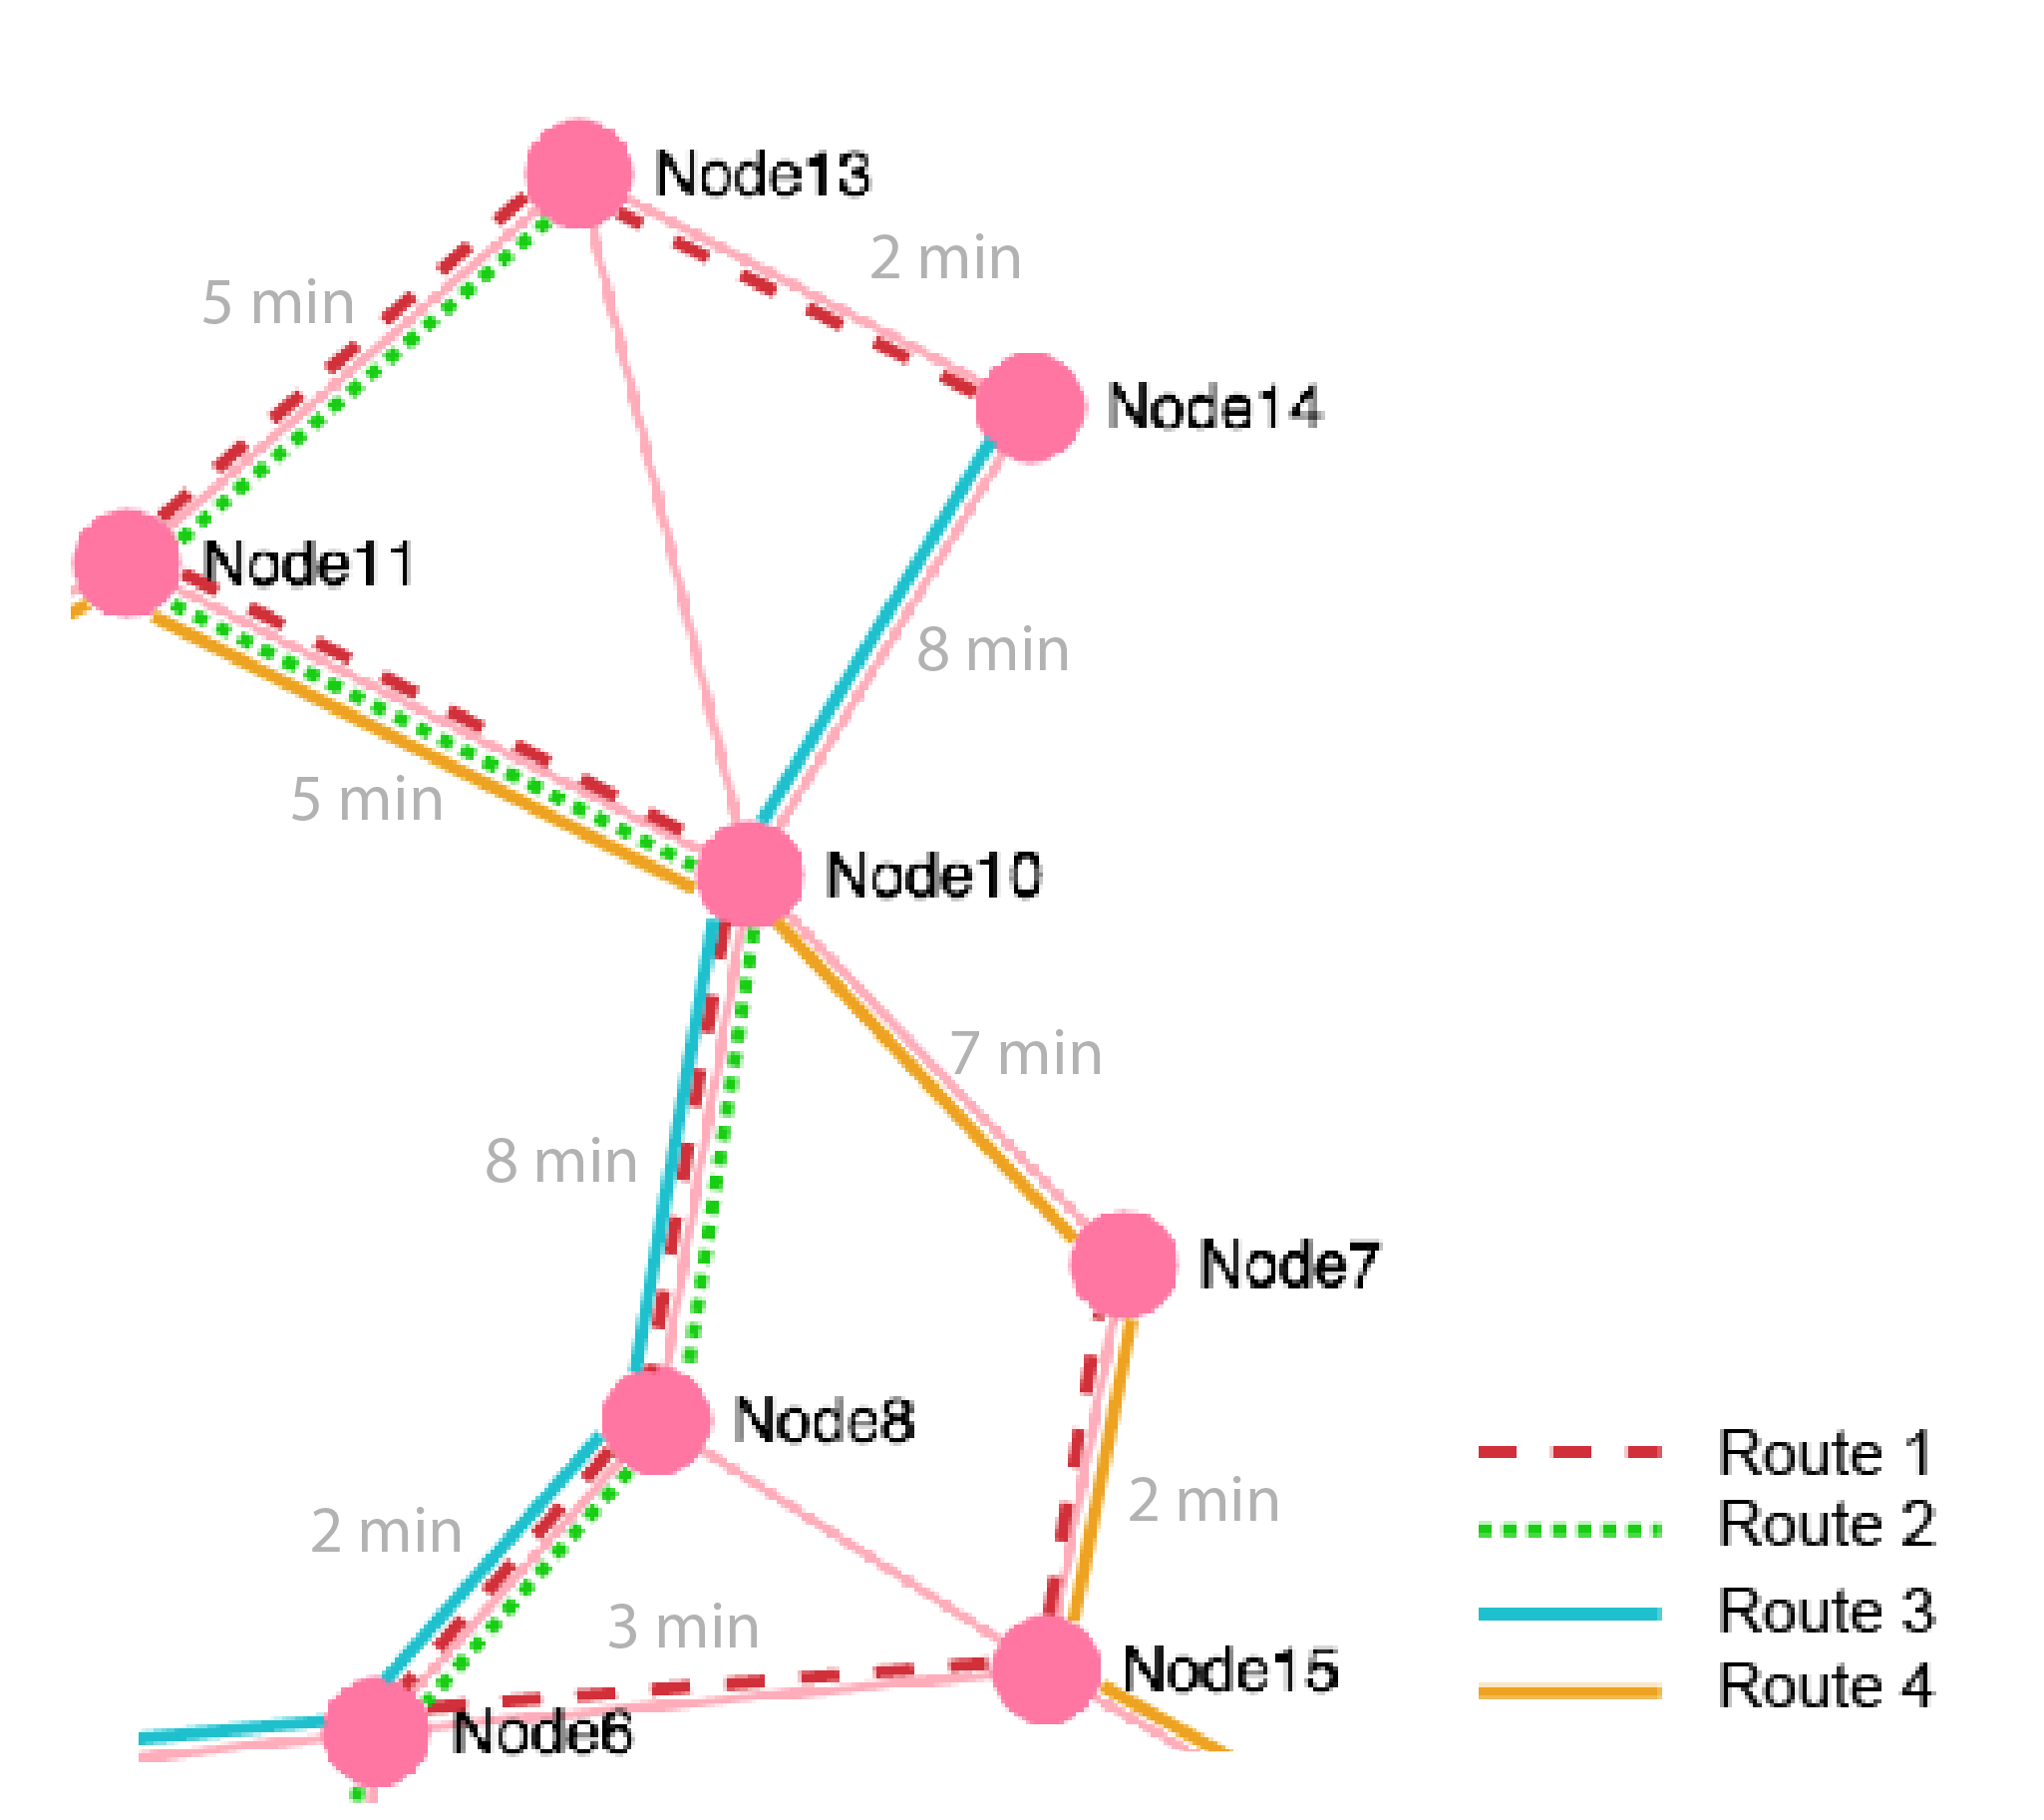
\includegraphics[width=3.5in]{assets/mandl_withTT_utsnitt.png}
    \end{center}
    \caption{A fragment of the best route set, having four route sets, constructed by the proposed algorithm including transfer times in minutes between each node.}
    \label{fig:mandlWithTT} 
\end{figure}

The best route set, having six routes, is presented in Fig. \vref{fig:bestRouteSet6}, the best route set, having seven routes, is presented in Fig. \vref{fig:bestRouteSet7}, and the best route set, having eight routes, is presented in Fig. \vref{fig:bestRouteSet8}. The performance comparison for each route set size is found in Table \vref{table:performanceComparison_6}, Table \vref{table:performanceComparison_7}, and Table \vref{table:performanceComparison_8}, respectively. As one can observe, in all route set sizes the proposed method is continuing to produce a higher $ATT$ than all other approaches, and performance criteria $d_0, d_1,$ and $d_{2}$ are all below average, whereas $d_{unsat}$ is still 0. %It is worth mentioning that neither of the algorithms we are comparing against (sjekke dette) tested their algorithms on other, larger networks. Their proposed algorithm could have been verified by also applying their algorithm to a larger test case.  
As one can observe in Table \vref{table:performanceComparison_routesets}, the amount of direct travelers increase, and the average travel time decrease in line with the number of routes. This corresponds to the growth in performance in all other approaches. The probability of finding direct routes and routes with a small travel time will be greater when there are more routes to select from. 

 \begin{table}[H]
    \centering
    \begin{tabular}{|l||l|l|l|l|l|}
    \hline
    Route Set & $d_0(\%)$ & $d_1(\%)$ & $d_2(\%)$ & $d_{unsat}(\%)$ & $ATT$ \\
    \hline
    4 & 85.21 & 13.49 & 1.30 & 0.00 & 10.27\\
    6 & 87.17 & 12.0 & 0.82 & 0.01 & 10.11\\
    7 & 88.49 & 10.72 & 0.79 & 0.0 & 10.08\\
    8 & 89.16 & 10.05 & 0.80 & 0.0 & 10.06\\
    \hline
    \end{tabular}
    \caption {Evaluating increase of Route Sets}
    % 50 runs
    \label{table:performanceComparison_routesets}
\end{table}








